\chapter{Extended Evaluation Examples}

This appendix collects worked evaluation examples that support the interpretation in Chapter 5. They are retained here as supplementary diagnostic material rather than part of the main final-report narrative.

\section{Stage-Separated Diagnostic Scenarios}
The evaluation framework separates retrieval quality from generation quality so that different failure modes can be interpreted more precisely.

\subsection{Retrieval Failure}
\begin{figure}[H]
  \centering
  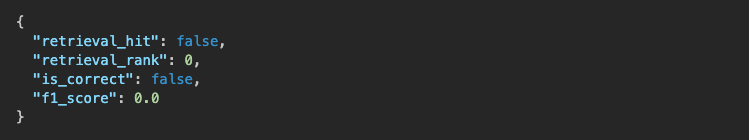
\includegraphics[width=1.0\textwidth]{figures/retrieval_failure_scenario_diagnostic_example.png}
  \caption{Retrieval failure scenario diagnostic example}
  \label{fig:fig57}
\end{figure}

In this case, the pipeline failed to retrieve any temporally relevant chunk. Such failures suggest that retriever configuration, fusion behavior, or reranking may need further adjustment.

\subsection{Generation Failure}
\begin{figure}[H]
  \centering
  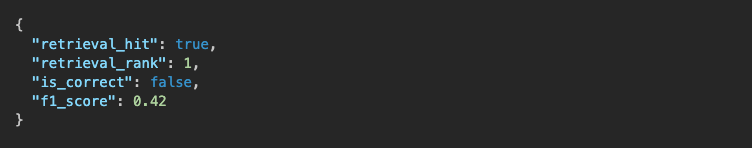
\includegraphics[width=1.0\textwidth]{figures/generation_failure_scenario_with_successful_retrieval.png}
  \caption{Generation failure scenario with successful retrieval}
  \label{fig:fig58}
\end{figure}

Here, retrieval succeeded but the answer-generation stage focused on the wrong aspect of the evidence. This type of failure is more likely to be addressed through prompt refinement, model choice, or context presentation.

\subsection{Perfect Performance}
\begin{figure}[H]
  \centering
  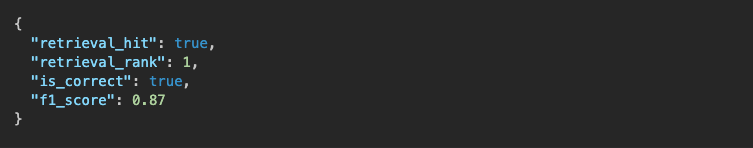
\includegraphics[width=1.0\textwidth]{figures/perfect_performance_scenario_for_both_retrieval_and_generation.png}
  \caption{Perfect performance scenario for both retrieval and generation}
  \label{fig:fig59}
\end{figure}

This case shows the intended behavior of the full pipeline: relevant evidence is retrieved at the top rank and the generated answer is both lexically and semantically aligned with the reference.

\section{Detailed Worked Examples}

\subsection{Success Case}
\begin{figure}[H]
  \centering
  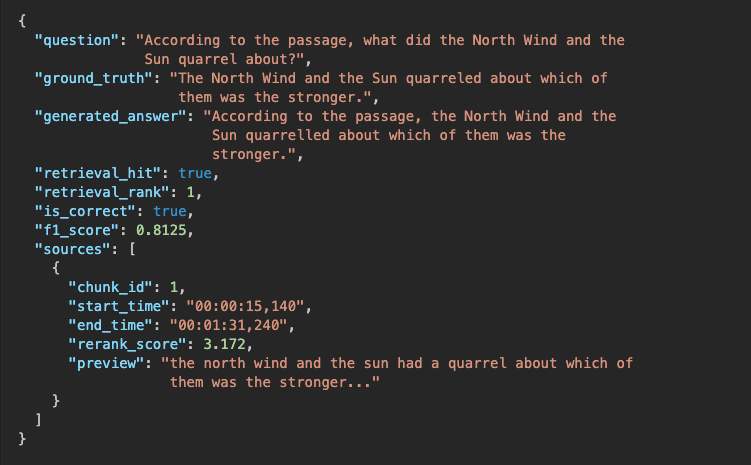
\includegraphics[width=1.0\textwidth]{figures/detailed_success_case_example_with_perfect_retrieval_and_generation.png}
  \caption{Detailed success case example with perfect retrieval and generation}
  \label{fig:fig64b}
\end{figure}

This example illustrates a strong end-to-end result, with the relevant chunk ranked first and the answer judged correct despite a minor spelling variation.

\subsection{Failure Case}
\begin{figure}[H]
  \centering
  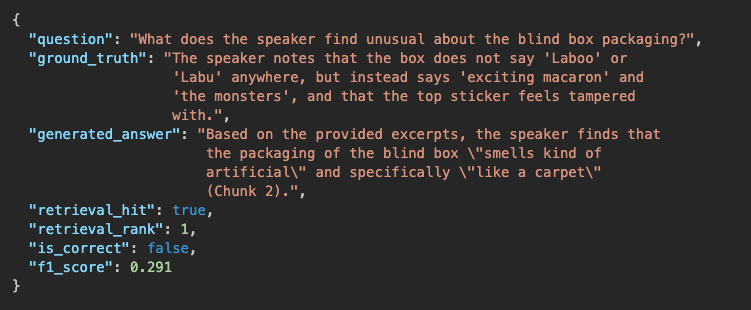
\includegraphics[width=1.0\textwidth]{figures/failure_case_example_with_retrieval_success_but_generation_error.png}
  \caption{Failure case example with retrieval success but generation error}
  \label{fig:fig65}
\end{figure}

This is a true generation error: the model had access to the relevant evidence but answered a secondary aspect of the question rather than the intended main point.

\subsection{False Negative Case}
\begin{figure}[H]
  \centering
  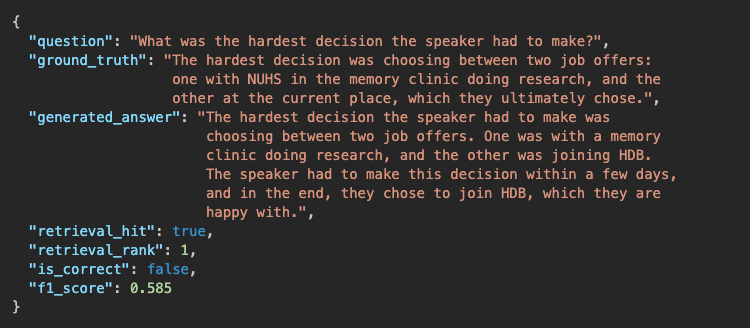
\includegraphics[width=1.0\textwidth]{figures/false_negative_example_with_more_specific_generated_answer.png}
  \caption{False negative example with more specific generated answer}
  \label{fig:fig66}
\end{figure}

In this case, the generated answer is more specific than the reference answer while remaining grounded in the transcript. The example highlights a limitation of the current judging setup, where semantically valid elaboration can still be marked as incorrect.
